\chapter{System Demonstrations and Implementation}
\label{chap:system_demos}

\section{Introduction}
\label{sec:system_demos:intro}
This chapter presents practical implementations of the methods which were discussed in the previous chapters. We are moving from theoretical foundations towards real-world applications; thereby, we demonstrate systems that illustrate how a combination of Large Language Models (LLMs) and Knowledge Graphs (KGs) can be utilized for addressing factoid question answering tasks. These developed implementations serve not only as a proof-of-concept for our methodological contributions but also represent usable tools for researchers and potential end-users in this field.
The demonstrated systems are the following:
\begin{itemize}
    \item A baseline sequence-to-sequence (Seq2Seq) model pipeline, which serves as a foundational T5-large-SSM-NQ model~\cite{DBLP:journals/corr/abs-1910-10683} for comparison.
    \item The M3M pipeline, this represents our original approach to KGQA as was presented in our paper~\cite{DBLP:conf/acl/RazzhigaevSMBP23}.
    \item The Answer Candidate Type (ACT) Selection pipeline, which corresponds to the methodologies discussed in Chapter~\ref{chap:act_selection}.
    \item A subgraph visualization tool, this was developed for supporting the research on controllable KG-LLM fusion presented in Chapter~\ref{chap:controllable_fusion}.
\end{itemize}
The main motivation behind these system demonstrations is related to the necessity of bridging the gap existing between theoretical advancements and practical utility. Through integration of LLMs with KGs, our aim is to enhance accuracy and reliability of question answering systems, especially for handling simple factoid questions across multiple domains and languages. This chapter draws specific inspiration from our research work "A System for Answering Simple Questions in Multiple Languages," where the M3M pipeline for the KGQA problem was presented~\cite{DBLP:conf/acl/RazzhigaevSMBP23}. This work focuses on leveraging structured knowledge for improvement of language model performance in diverse linguistic contexts.

All source code for the systems which are demonstrated in this chapter can be found at \url{https://github.com/s-nlp/m3m}.

This chapter's organization consists of several sections in order to provide a comprehensive overview of our system demonstrations. Each section is focused on a specific aspect of the implementation, from its design to evaluation, thereby ensuring a clear understanding of how these systems operate in real-world scenarios. A brief overview of each section is provided below:

% <-- TODO

\begin{itemize}
    \item \textbf{System Architecture (Section \ref{sec:system_demos:architecture}):} This section provides an outline of the general architecture of our implemented systems. It details the integration of LLMs with KGs, and also the specific components of the M3M pipeline, the ACT Selection pipeline, the baseline Seq2Seq model, and the subgraph visualization tool.
    \item \textbf{Implementation Details (Section \ref{sec:system_demos:implementation}):} Here, we will delve into technical specifics of our systems' implementation. This includes the selection of technologies, programming frameworks (for instance, FastAPI for API endpoints), key Python libraries (e.g., PyTorch, spaCy, Sentence Transformers, PyWikidata), and also challenges that were faced during development, particularly in ensuring cross-linguistic compatibility and efficient KG interaction.
\end{itemize}

\section{System Architecture}
\label{sec:system_demos:architecture}
This section describes the overarching design of our implemented question answering systems and the accompanying visualization tool. Each system leverages a combination of LLMs and KGs, but with distinct architectural focuses reflecting their specific research contributions.

\subsection{Baseline Seq2Seq Pipeline}
\label{sec:system_demos:architecture:seq2seq}
This pipeline provides a standard sequence-to-sequence LLM functionality, primarily using T5-like models. Its architecture is straightforward:
\begin{enumerate}
    \item It uses a pre-trained Seq2Seq model. The \path{build\_seq2seq\_pipeline} function (referenced in \path{m3m/app/pipelines/seq2seq.py}) is responsible for loading the model and its tokenizer from a specified path. This typically involves using the HuggingFace \path{transformers}\footnote{\url{https://huggingface.co/docs/transformers/}} library, specifically classes like \path{AutoTokenizer.from_pretrained} to load the tokenizer and \path{AutoModelForSeq2SeqLM.from_pretrained} to load the pre-trained weights of a T5-like model. The model is then moved to the appropriate \path{torch.device} (CPU or GPU) as specified in the configuration.
    \item Given an input question, the text is first tokenized using the loaded tokenizer, converting it into a format suitable for the model (e.g., input IDs, attention mask).
    \item The model's \path{generate()} method is then called with these tokenized inputs to produce a sequence of output token IDs representing the potential answer(s). This method often incorporates beam search or other decoding strategies to generate a list of candidates.
    \item These output token IDs are subsequently decoded back into human-readable text strings using the tokenizer's \path{batch_decode()} or \path{decode()} method.
    \item These generated textual labels are then mapped to Wikidata entity identifiers using \path{label_to_entity_idx}.
\end{enumerate}
This pipeline serves as a fundamental component for generating initial answer candidates in the ACT Selection pipeline and acts as a baseline for comparing the performance of more sophisticated KG-fused methods. It is accessible via the \path{/pipeline/seq2seq/} FastAPI endpoint (see Figure~\ref{fig:demo_seq2seq}).

\begin{figure}[htb]
    \centering
    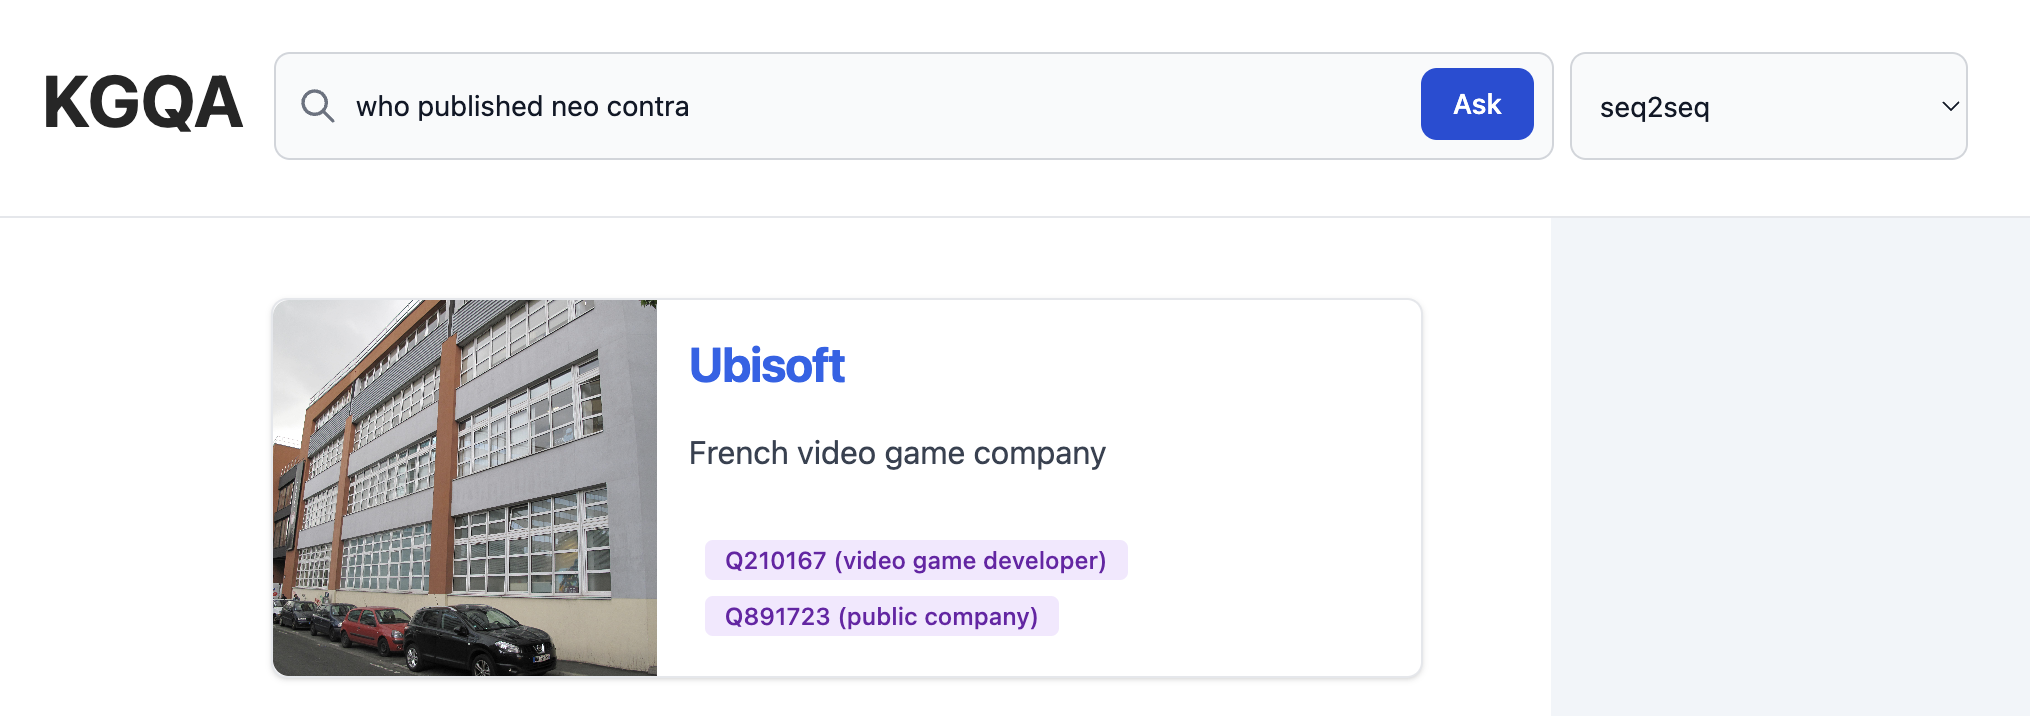
\includegraphics[width=0.99\textwidth]{system_demonstration/demo_seq2seq.png}
    \caption{Demonstration of the baseline Seq2Seq pipeline.}
    \label{fig:demo_seq2seq}
\end{figure}

\subsection{M3M Pipeline}
The M3M pipeline, corresponding to our work in~\cite{DBLP:conf/acl/RazzhigaevSMBP23}, is engineered for retrieving answers from a Knowledge Graph by deeply matching semantic representations of the question with KG entities and relations (an example is shown in Figure~\ref{fig:demo_m3m}). Its architecture integrates several custom modules:

\begin{itemize}
    \item \textbf{Linguistic Preprocessing}:
    \begin{itemize}
        \item \path{NounsExtractor}: This module is responsible for identifying key candidate entities within the input question. It employs a hybrid approach, utilizing the Natasha\footnote{\url{https://github.com/natasha/natasha}} library for robust named entity recognition and morphological analysis in Russian and other languages, and spaCy\footnote{\url{https://spacy.io/}} for English. It also handles phrases within quotes and performs normalization using a custom \path{KostilPhraseNormalization} module (which itself uses Natasha's morphological tools) to standardize noun phrases. If primary NER fails, it falls back to extracting nouns and bigrams.
        \item The \path{M3MQAmatching} variant extends this with broader entity extraction using spaCy's multilingual and English NER models (\path{xx_ent_wiki_sm} and \path{en_core_web_trf}).
    \end{itemize}
    \item \textbf{Knowledge Graph Interaction and Candidate Retrieval}:
    \begin{itemize}
        \item Initial question entities (derived from extracted nouns/entities) are searched against Wikidata using \path{get_wd_search_results} to obtain their Wikidata QIDs.
        \item A local \path{wikidata_cache} (pre-populated, likely containing 1-hop or 2-hop neighborhoods of frequent entities) is queried to find connected entities and properties. This forms a candidate set of (subject, property, object) triples.
        \item The \path{M3MQAmatching} variant additionally uses a LevelDB\footnote{\url{https://github.com/google/leveldb}} instance (\path{plyvel}) to store and retrieve aliases for Wikidata entities (\path{aliases_db}), aiding in matching question entities to KG subjects.
    \end{itemize}
    \item \textbf{Semantic Representation and Matching Core (M3MQA class)}:
    \begin{itemize}
        \item \path{EncoderBERT}: A BERT-based encoder (\path{bert-base-multilingual-cased}) fine-tuned for this task. It takes the tokenized question and generates a dense vector representation (question embedding).
        \item \textbf{Projection Layers}: Separate trainable projection heads (\path{projection_E}, \path{projection_Q}, \path{projection_P}) are applied to the question embedding. These layers transform the general question embedding into specialized representations tailored for matching against subject entities (E), object entities (Q), and properties (P) of KG triples, respectively.
        \item \textbf{Precomputed Embeddings}: The system loads precomputed embeddings for a large set of Wikidata entities (\path{embeddings_tensor_Q}) and properties (\path{embeddings_tensor_P}), along with mappings from their QIDs/PIDs to tensor indices (\path{id2ind}, \path{p2ind}).
        \item \textbf{Scoring Mechanism}: For each candidate triple (E, P, Q) retrieved from the KG cache:
        \begin{enumerate}
            \item Cosine similarity is calculated between the projected question embedding for subjects and the embedding of \textbf{E}.
            \item Cosine similarity is calculated between the projected question embedding for objects and the embedding of \textbf{Q}.
            \item Cosine similarity is calculated between the projected question embedding for properties and the embedding of \textbf{P}.
            \item These three similarity scores, after a Softmax transformation, are aggregated (summed) to produce a final score for the triple.
        \end{enumerate}
        \item In the \path{M3MQAmatching} variant, an additional matching\_object\_to\_question\_score is computed. This score quantifies the lexical overlap between the labels/aliases of the first-hop entity (subject E) in a candidate triple and the entities directly extracted from the input question. This score is added to the aggregated cosine similarities to further refine ranking, ensuring the KG subject is relevant to the question's focus.
    \end{itemize}
    \item \textbf{Output Generation}:
    \begin{itemize}
        \item The triples are ranked based on their aggregated scores.
        \item The system returns the top-k object entities (potential answers), their scores, the corresponding triples, and an "Uncertainty Estimation" (UE) score (typically the difference between the top two answer scores).
    \end{itemize}
\end{itemize}
The M3M pipeline exposes its functionality via a FastAPI endpoint (\path{/pipeline/m3m/}), taking a question string and returning a structured JSON response, as illustrated in Figure~\ref{fig:demo_api_m3m}. The \path{M3MQAmatching} variant provides enhanced entity matching capabilities through its specific endpoint (\path{/m3m_subj_question_matching/}).

\begin{figure}[htb]
    \centering
    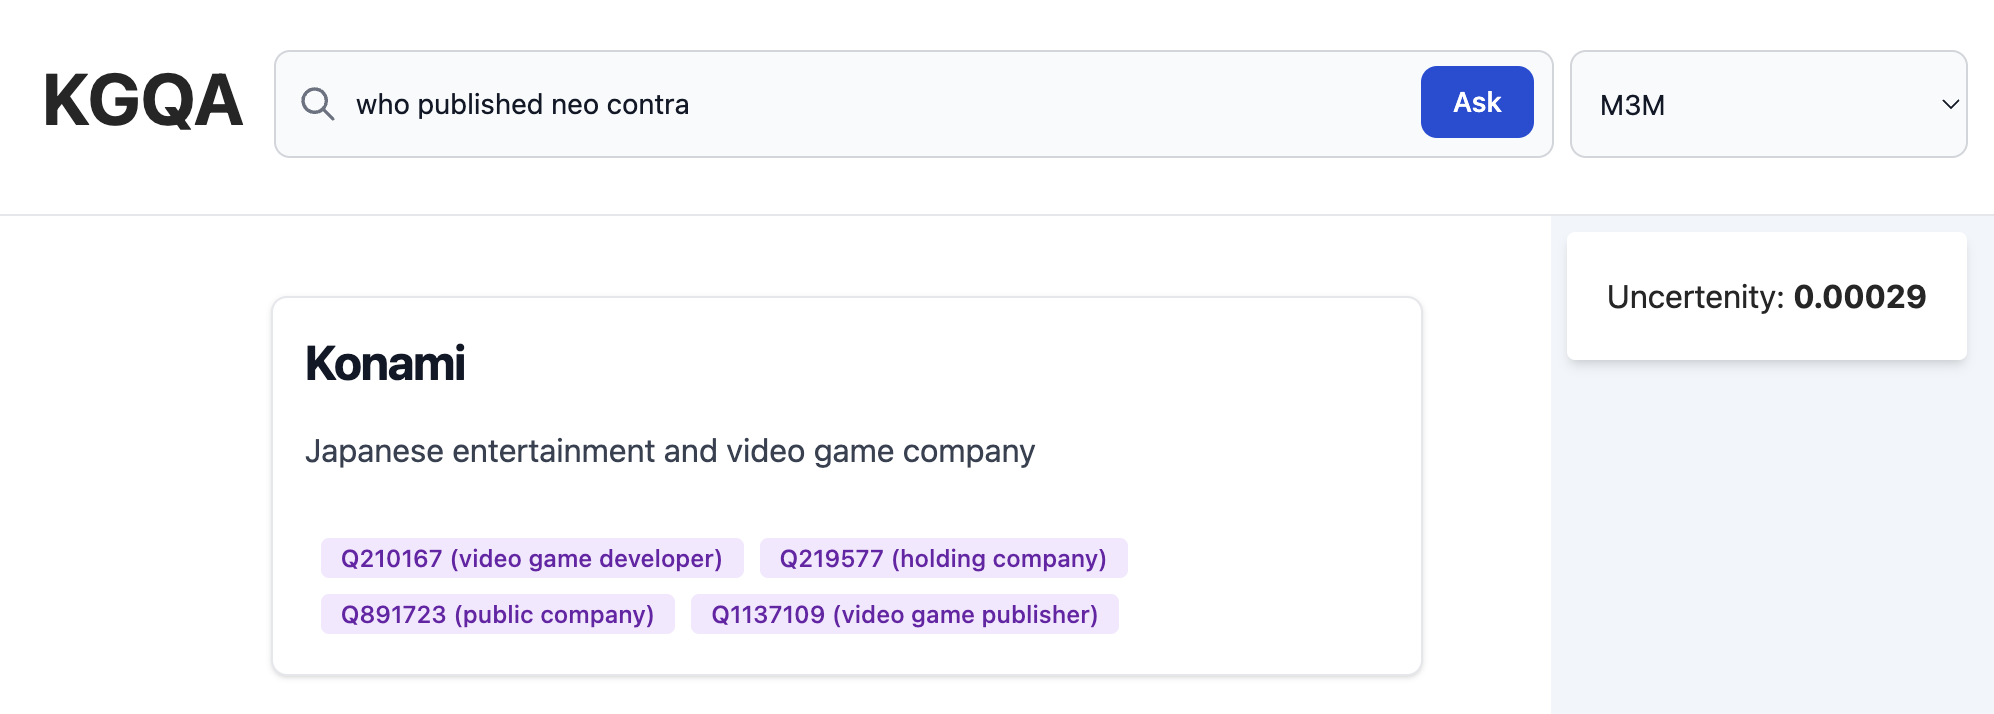
\includegraphics[width=0.99\textwidth]{system_demonstration/demo_m3m.png}
    \caption{Demonstration of the M3M pipeline in action.}
    \label{fig:demo_m3m}
\end{figure}

\begin{figure}[htb]
    \centering
    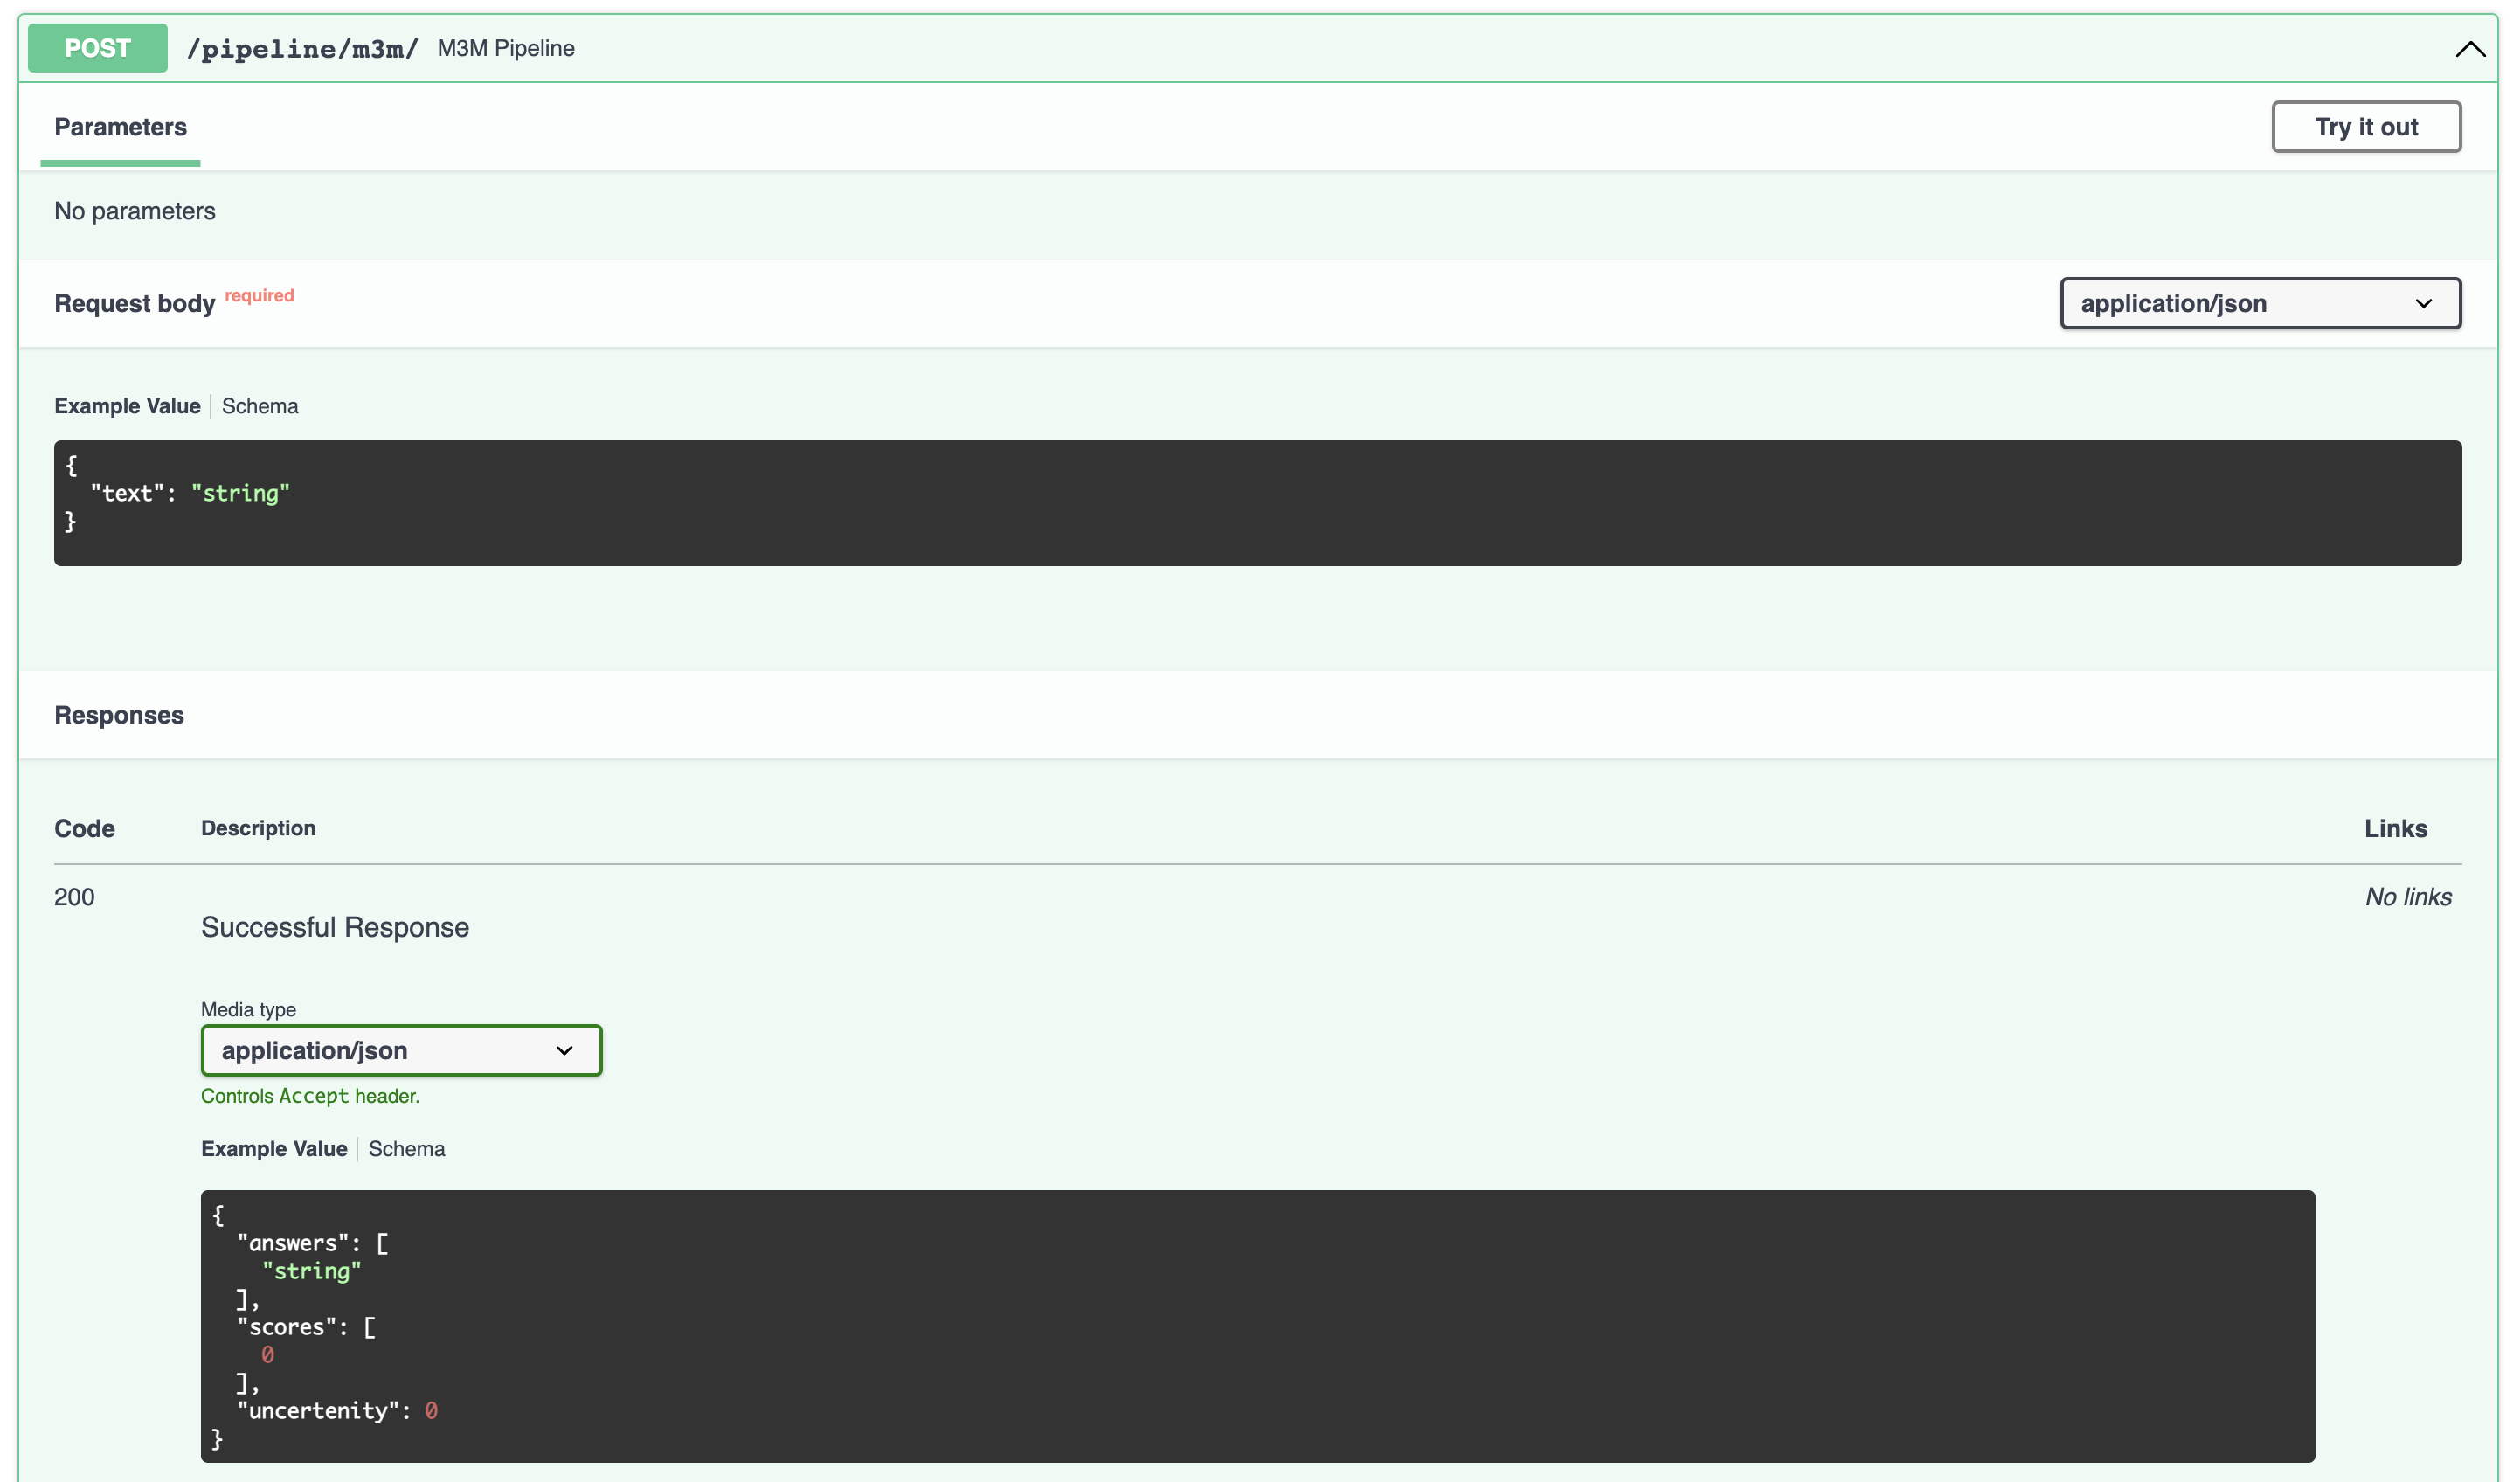
\includegraphics[width=0.99\textwidth]{system_demonstration/demo_api_m3m.png}
    \caption{API interaction with the M3M pipeline.}
    \label{fig:demo_api_m3m}
\end{figure}

\subsection{Answer Candidate Type (ACT) Selection Pipeline}
The ACT Selection pipeline, implemented in \path{m3m/app/pipelines/act_selection.py}, implements the methodologies discussed in Chapter~\ref{chap:act_selection}. This system refines the KGQA process by robustly identifying the semantic type of the expected answer (demonstrated in Figure~\ref{fig:demo_act}). Its architecture involves several key components and processing steps:
\begin{enumerate}
    \item \textbf{Named Entity Recognition (NER):} Utilizes a \path{NerToSentenceInsertion} module (based on spaCy) to identify entities in the input question.
    \item \textbf{Entity Linking:} Employs \path{mgenre} (Multilingual GENRE) for robust entity linking~\cite{decao2021multilingual}, followed by an \path{EntitiesSelection} step to refine linked entities. Wikidata search results (\path{get\_wd\_search\_results}) are used to map labels to KG identifiers.
    \item \textbf{Initial Answer Candidate Generation:} A baseline Seq2Seq model (see Section~\ref{sec:system_demos:architecture:seq2seq}) generates initial textual answer candidates. These are then linked to KG entities.
    \item \textbf{Candidate Ranking:} The core of this pipeline lies in the \path{QuestionToRankInstanceOf}, \path{QuestionToRankInstanceOfSimple}, and \path{QuestionToRankInstanceOfSimpleWithDescriptionMatching} classes. These classes score answer candidates based on a combination of factors, including:
    \begin{itemize}
        \item Semantic type matching (instance of scores).
        \item KG neighborhood information (forward one-hop neighbors score).
        \item Scores from the initial Seq2Seq model.
        \item Similarity between question and KG properties.
    \end{itemize}
\end{enumerate}
This pipeline is also exposed via FastAPI through multiple endpoints (e.g., \path{/pipeline/act_selection/main}, \path{/simple_type_selection/}, \path{/simple_with_description_qustion_similarity_type_selection/}), each offering slightly different ranking strategies and response structures tailored to the specific ACT selection variant (see Figure~\ref{fig:demo_m3m_act_1} for an example of its integration).  

\begin{figure}[htb]
    \centering
    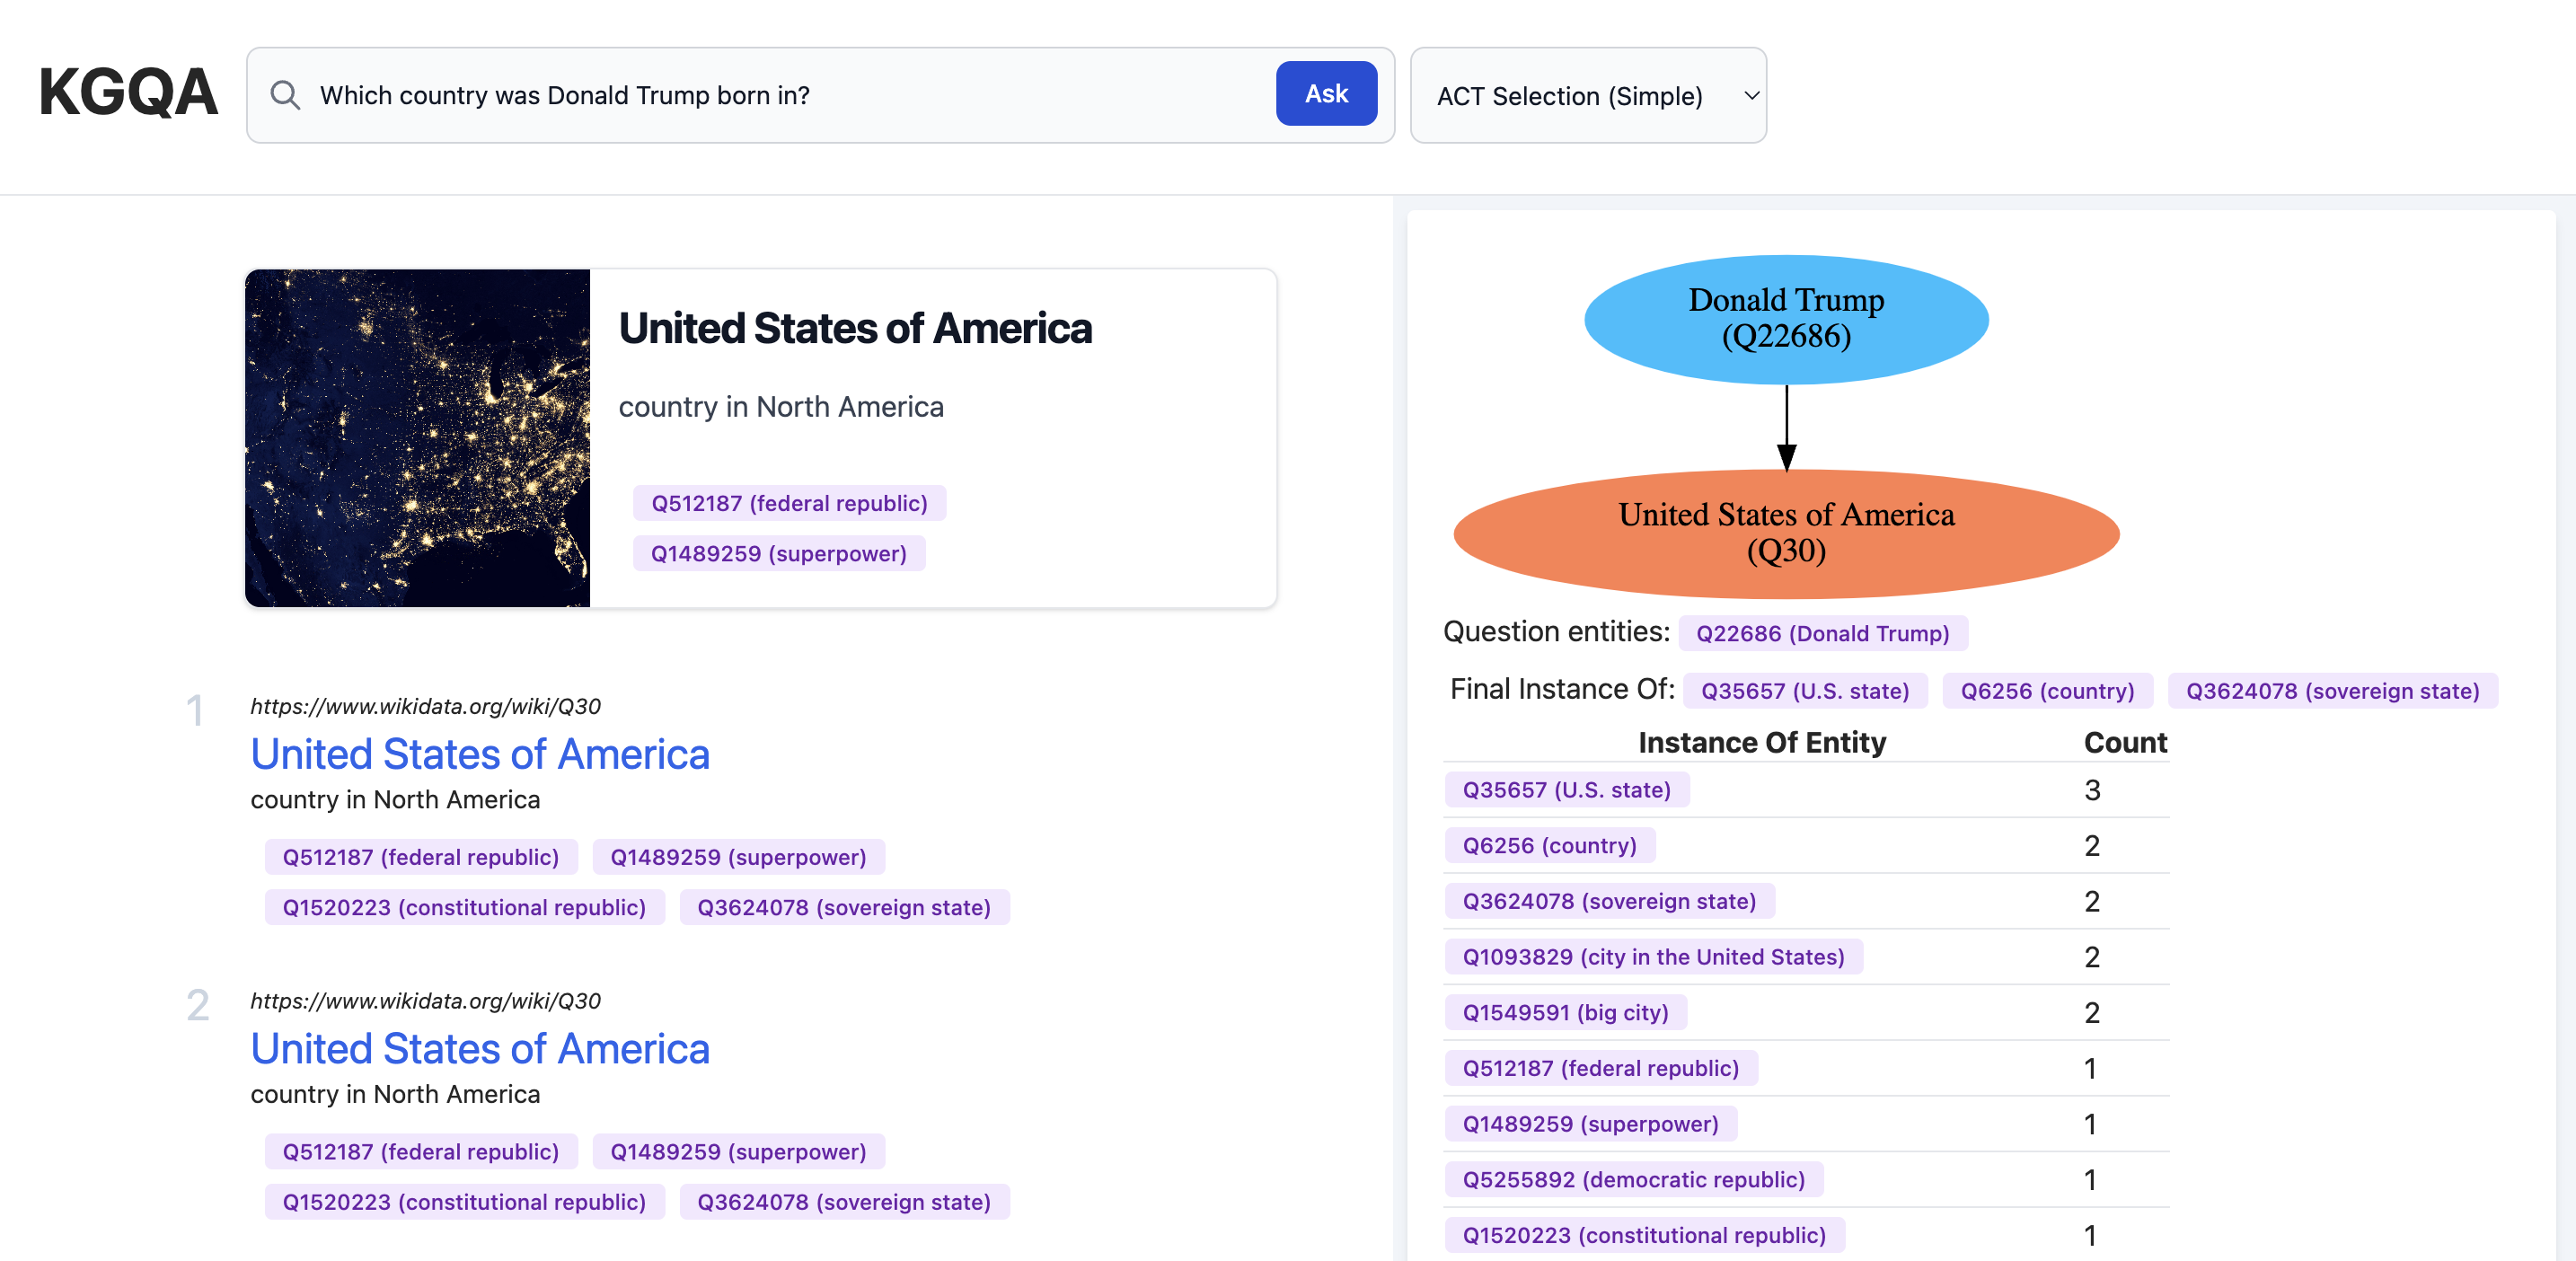
\includegraphics[width=0.99\textwidth]{system_demonstration/demo_act.png}
    \caption{Demonstration of the ACT Selection pipeline.}
    \label{fig:demo_act}
\end{figure}

\begin{figure}[htb]
    \centering
    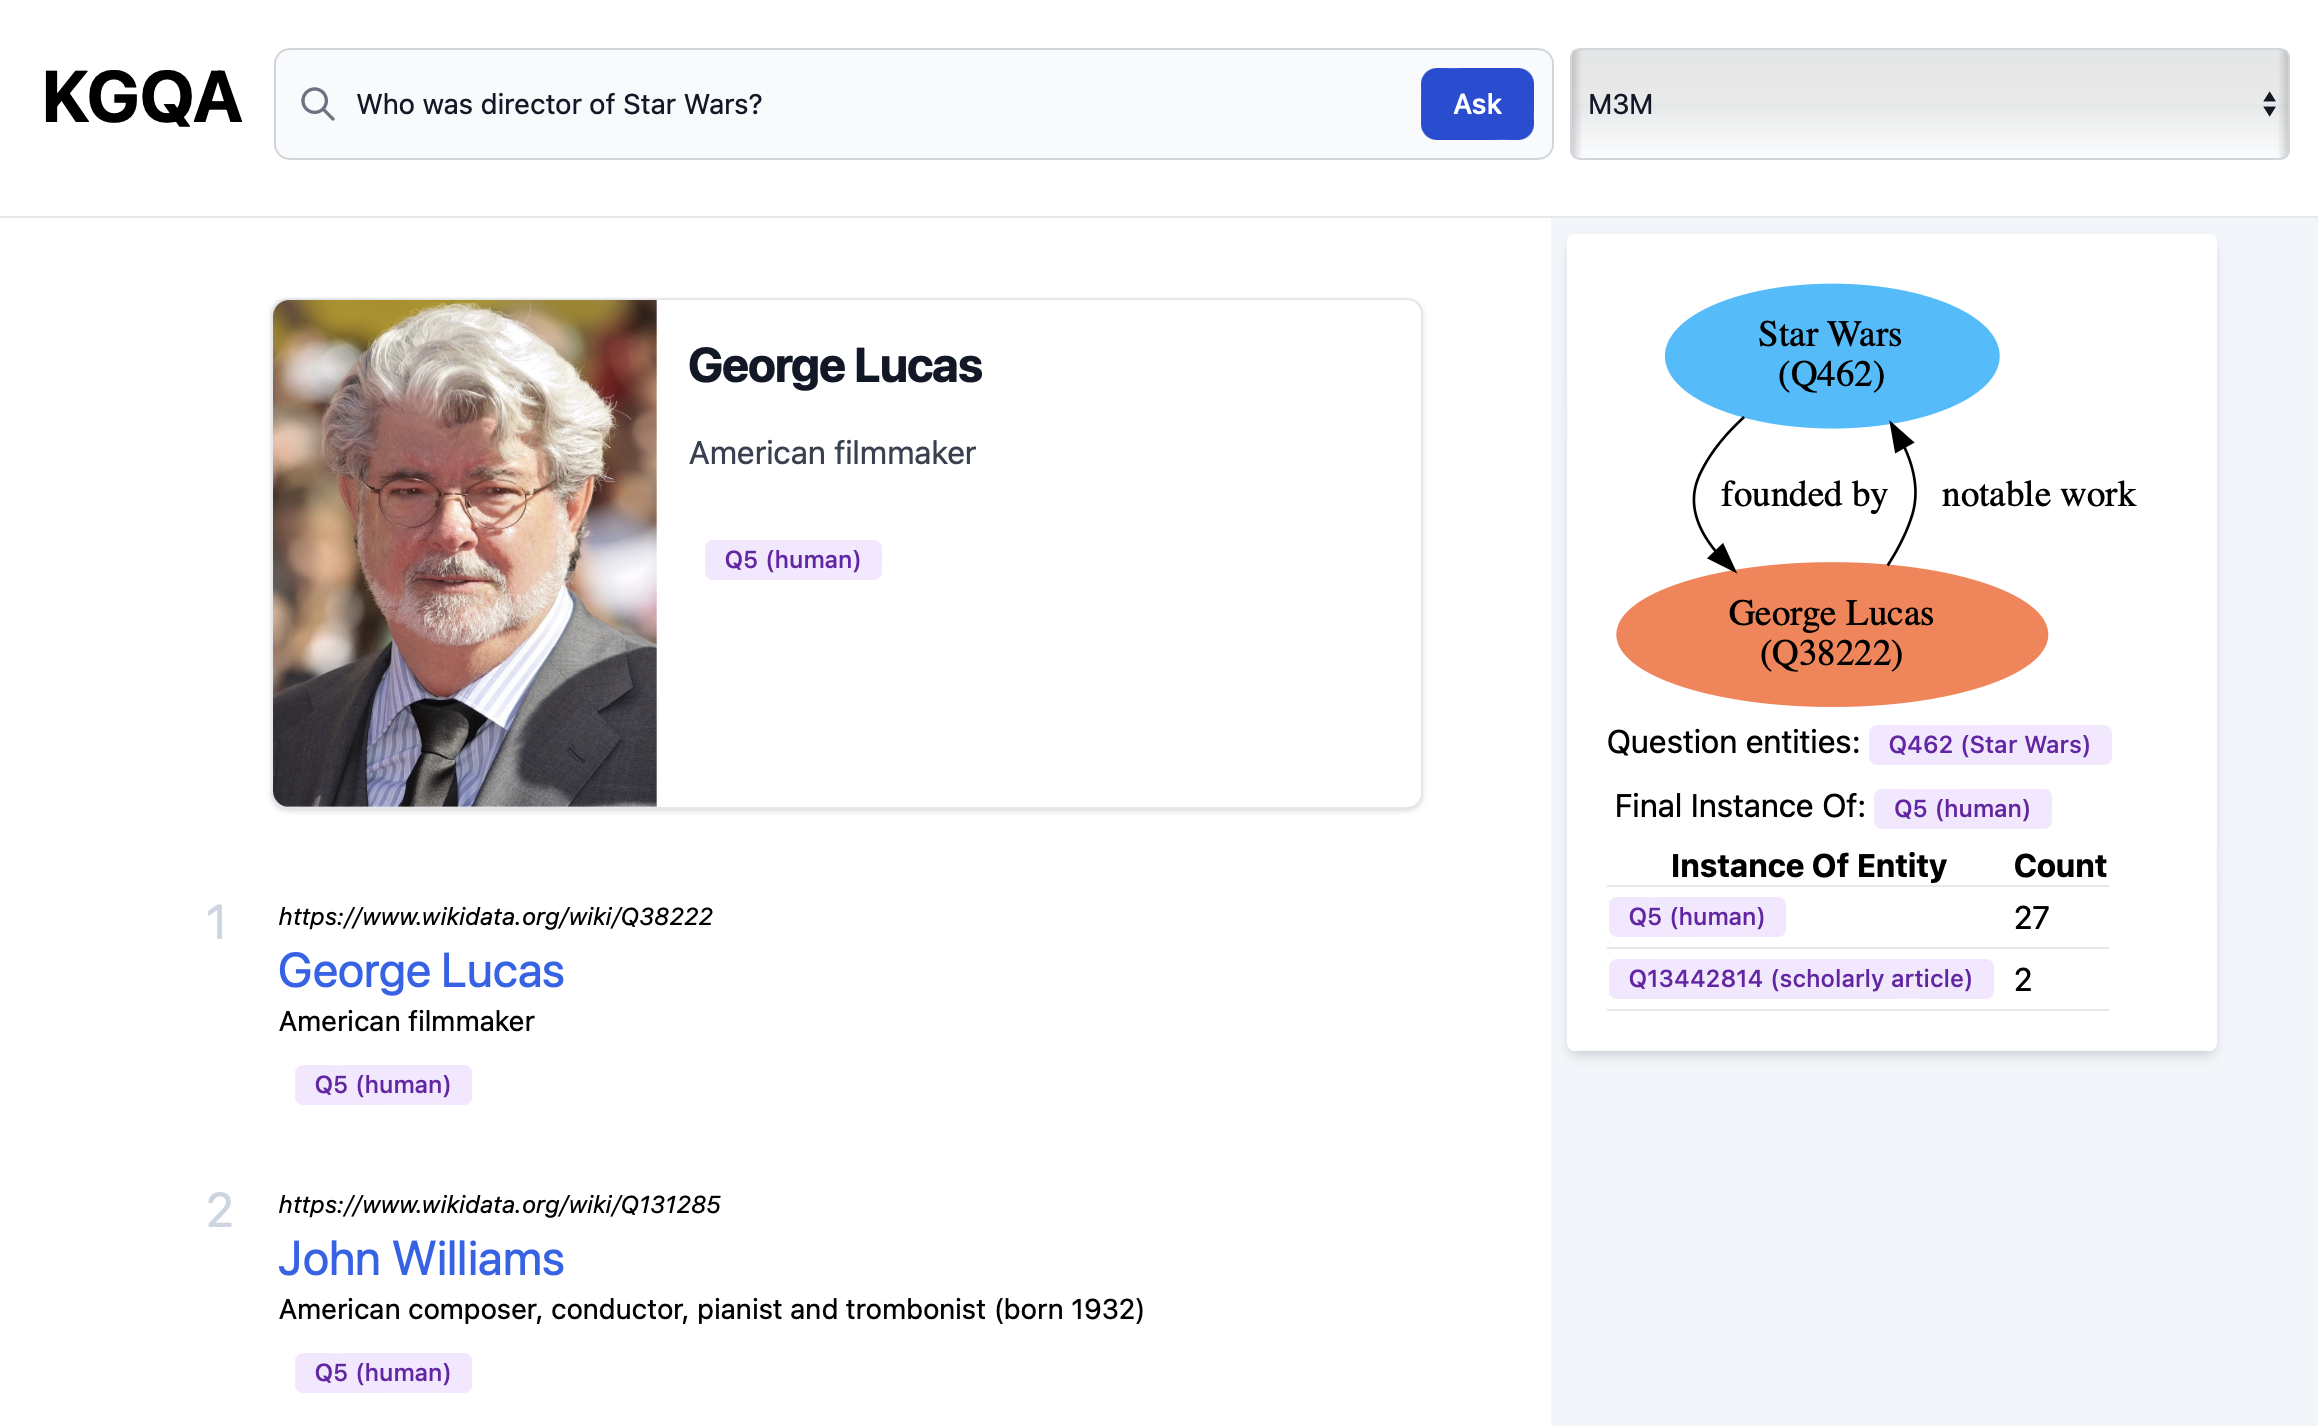
\includegraphics[width=0.99\textwidth]{system_demonstration/demo_m3m(act)_1.png}
    \caption{Further demonstration of the M3M pipeline incorporating ACT Selection principles.}
    \label{fig:demo_m3m_act_1}
\end{figure}

\subsection{Subgraph Visualization Tool}
The subgraph visualization tool, with its frontend defined in \path{m3m/app/templates/graph_visualise.html}, is designed to support the research presented in Chapter~\ref{chap:controllable_fusion} by allowing interactive exploration of KG subgraphs. Its architecture is web-based:
\begin{enumerate}
    \item \textbf{User Input:} The user provides question entities and an answer entity (e.g., "Q2, Q3 -> Q4").
    \item \textbf{Backend API Calls:} JavaScript (using jQuery) makes asynchronous calls to backend FastAPI endpoints (likely under \path{/wikidata/entities/ssp/graph/}) that is implemented as it was described in Chapter~\ref{chap:controllable_fusion} to:
    \begin{itemize}
        \item Fetch an SVG representation of the shortest path subgraph between the specified entities.
        \item Retrieve textual descriptions of the subgraph generated by different Graph2Text models (T5-XL and GAP, as indicated in the HTML).
    \end{itemize}
    \item \textbf{Frontend Rendering:}
    \begin{itemize}
        \item The SVG graph is rendered using D3.js.
        \item Textual descriptions are displayed alongside the graph.
        \item Interactive features include image previews for entities on mouseover.
    \end{itemize}
\end{enumerate}
This tool aids in understanding the connections within KGs and evaluating the quality of Graph2Text verbalizations, which are crucial for the controllable fusion methods.

\section{Implementation Details}
\label{sec:system_demos:implementation}
This section delves into the technical specifics of the implemented systems, highlighting the programming languages, frameworks, and key libraries that underpin their functionality. All backend pipelines are developed in Python and exposed as REST APIs using the FastAPI framework, facilitating modularity and ease of integration (an overview of the API interactions is provided in Figure~\ref{fig:demo_api}).

\begin{figure}[htb]
    \centering
    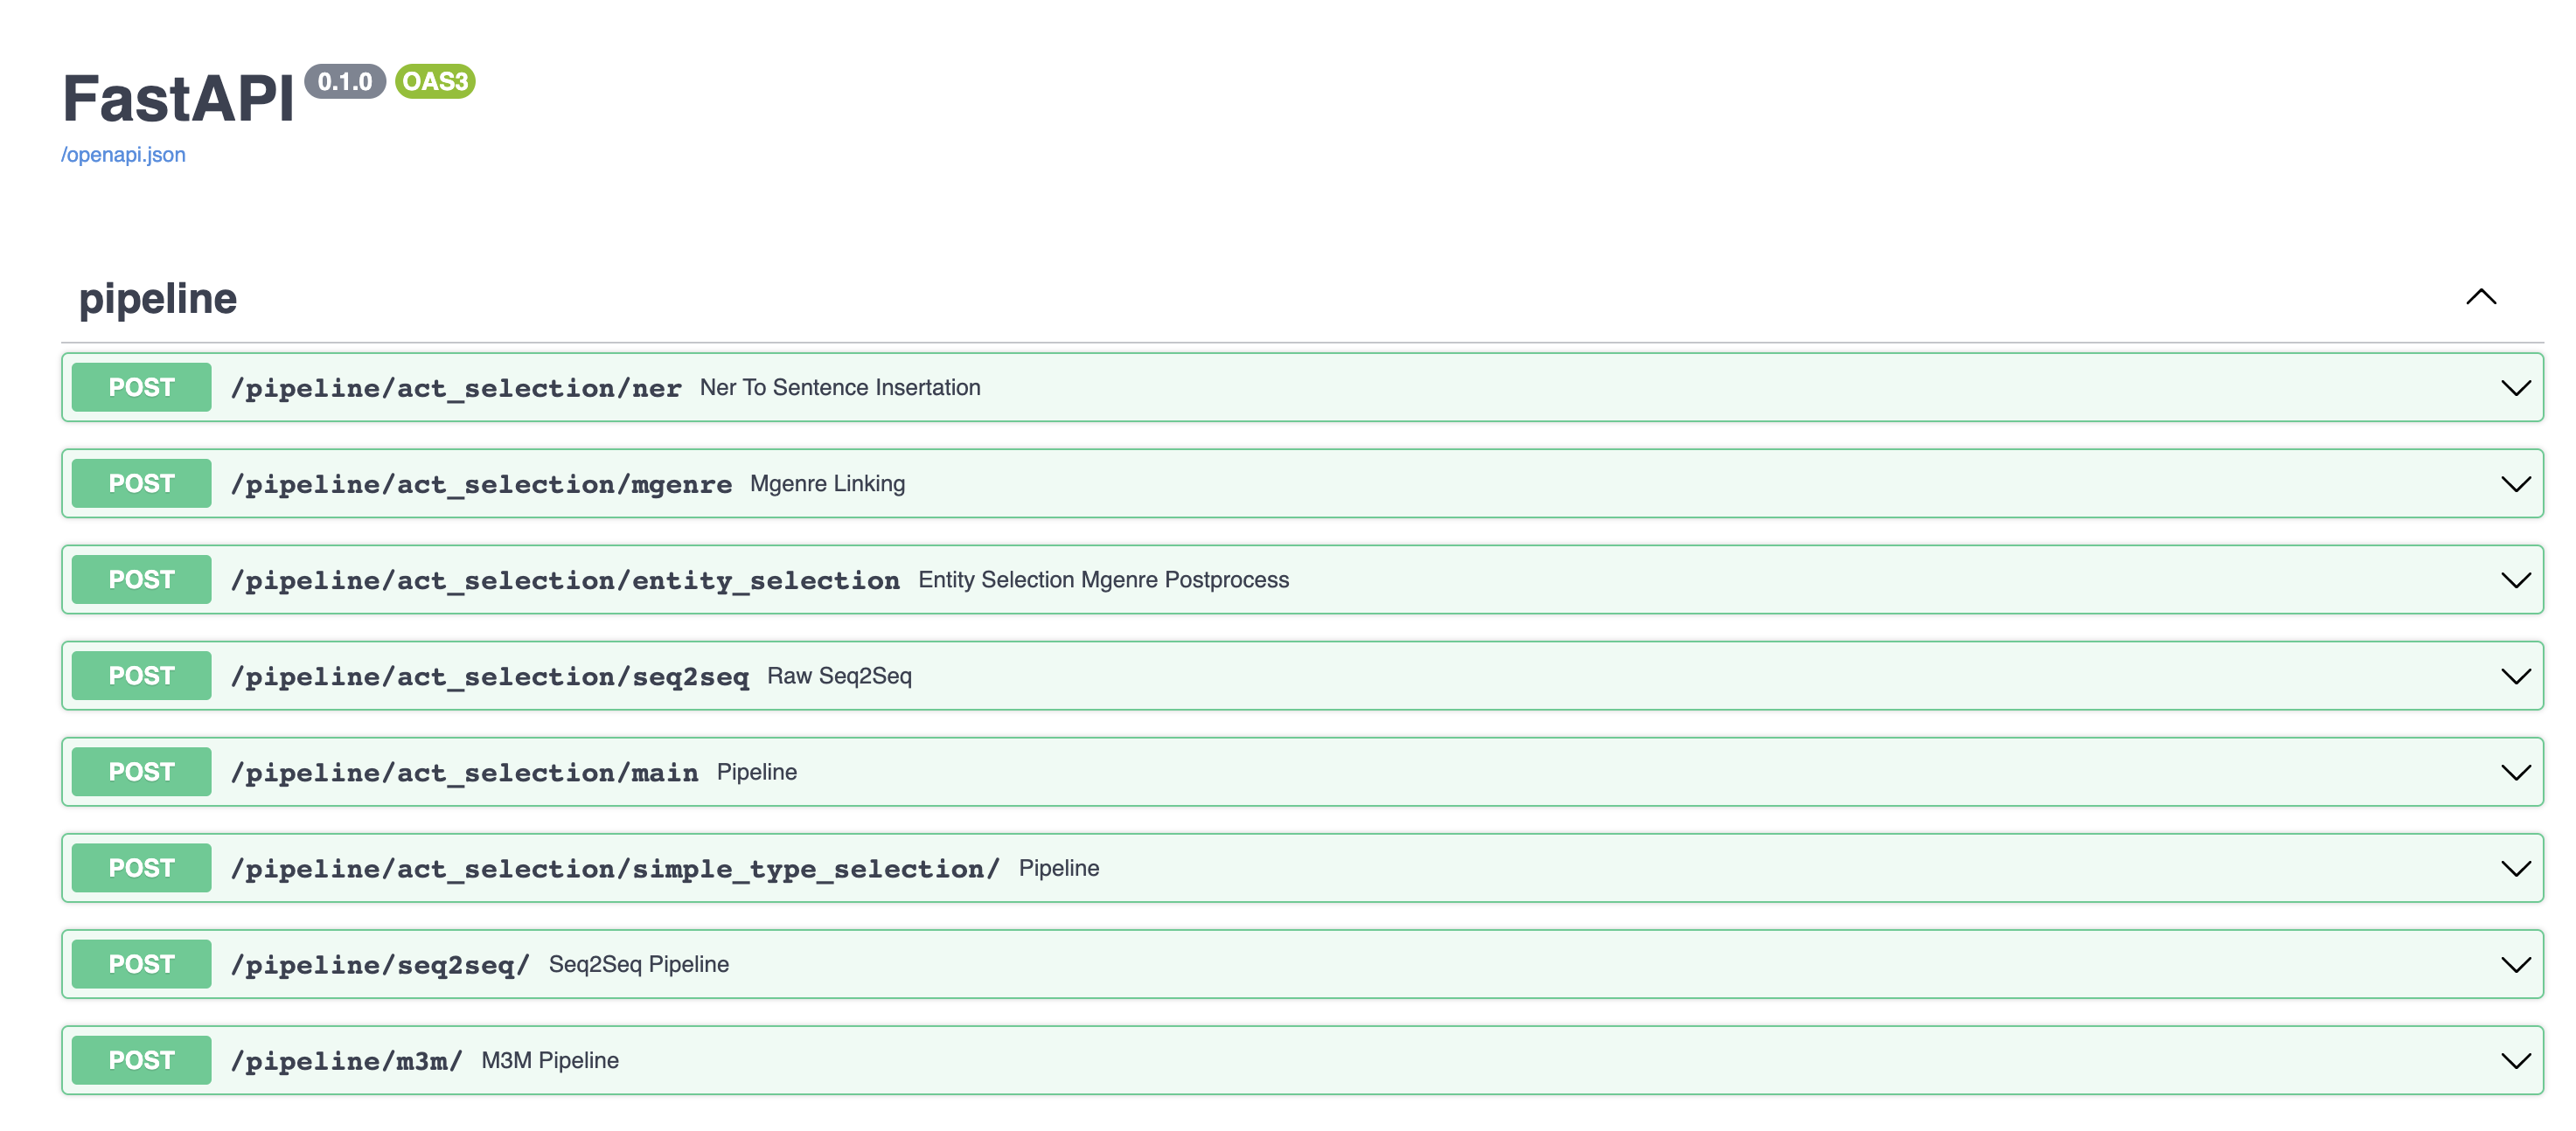
\includegraphics[width=0.99\textwidth]{system_demonstration/demo_api.png}
    \caption{Overview of the general API interface for the demonstrated systems.}
    \label{fig:demo_api}
\end{figure}

\subsection{M3M Pipeline Implementation}
The M3M pipeline (\path{m3m/app/kgqa/m3m.py}) leverages several powerful libraries for its KGQA tasks:
\begin{itemize}
    \item \textbf{KG Interaction:} \path{pywikidata} is used for interacting with Wikidata to retrieve entity information and triples. \path{plyvel} is employed for efficient local storage and retrieval, likely for caching KG data or precomputed embeddings.
    \item \textbf{Natural Language Processing:} \path{spacy} is utilized for initial text processing tasks. For semantic understanding and similarity calculations, \path{sentence-transformers} (specifically models like \path{EncoderBERT} which is a component of \path{M3MQA}) and direct \path{cosine\_similarity} from \path{sklearn.metrics.pairwise} are used. \path{langdetect} is included for language identification, and \path{nltk.corpus.stopwords} for text normalization.
    \item \textbf{Machine Learning Core:} \path{torch} serves as the foundational deep learning framework, particularly for the BERT-based components. \path{numpy} is used for numerical operations, especially in handling scores and arrays of results.
    \item \textbf{API and Concurrency:} \path{FastAPI} is used to define the API routes. \path{joblib} (Parallel, delayed) suggests optimizations for parallel processing of certain tasks within the pipeline. The \path{functools.lru\_cache} is used to cache results of frequently called functions, improving performance.
    \item \textbf{Configuration and Models:} The system relies on a configuration file (\path{app.config.m3m}) to load parameters for the \path{M3MQA} and \path{M3MQAmatching} core modules. Custom data models like \path{M3MPipelineResponce} and \path{QuestionRequest} (from \path{app.models.base}) define the structure of API inputs and outputs.
\end{itemize}

\subsection{ACT Selection Pipeline Implementation}
The ACT Selection pipeline (\path{m3m/app/pipelines/act_selection.py}) integrates various modules for advanced entity linking and type-based candidate ranking:
\begin{itemize}
    \item \textbf{Entity Processing Core:} It uses \path{NerToSentenceInsertion} (custom module likely located in \path{app.kgqa.ner}, using a model from \path{/data/ner/}) for NER. Multilingual entity linking is handled by \path{mgenre} (from \path{app.kgqa.mgenre}), built using \path{build_mgenre_pipeline}. \path{EntitiesSelection} (from \path{app.kgqa.entity_linking}) refines these entities. \path{pywikidata} (via \path{get_wd_search_results} from \path{app.kgqa.utils.utils}) is used for mapping textual labels to Wikidata entities.
    \item \textbf{Ranking Logic:} The core ranking is performed by classes like \path{QuestionToRankInstanceOf}, \path{QuestionToRankInstanceOfSimple}, and \path{QuestionToRankInstanceOfSimpleWithDescriptionMatching} (from \path{app.kgqa.act\_selection}).
    \item \textbf{Seq2Seq Integration:} It utilizes a Seq2Seq component (\path{app.pipelines.seq2seq.seq2seq}) for generating initial answer candidates.
    \item \textbf{API and Data Structures:} \path{FastAPI} exposes the various pipeline functionalities. Custom Pydantic models like \path{ACTPipelineResponce}, \path{QuestionEntitiesResponce}, etc. (from \path{app.models.base}) manage the structured data exchange.
    \item \textbf{Performance:} \path{joblib.Parallel} is used for parallelizing operations like fetching search results for multiple candidates. \path{functools.lru\_cache} is applied to API endpoints for caching, enhancing responsiveness.
\end{itemize}

\subsection{Baseline Seq2Seq Pipeline Implementation}
The baseline Seq2Seq pipeline (\path{m3m/app/pipelines/seq2seq.py}) is a more focused implementation:
\begin{itemize}
    \item \textbf{Core Model:} It relies on a T5-like model loaded via \path{build_seq2seq_pipeline} (from \path{app.kgqa.seq2seq}), which takes a model path and a \path{torch.device} from a configuration file (\path{app.config.seq2seq}).
    \item \textbf{Output Processing:} Generated textual labels are converted to Wikidata entity IDs using \path{label_to_entity_idx} (from \path{app.kgqa.utils.utils}), with parallel processing via \path{joblib.Parallel}.
    \item \textbf{API:} A \path{FastAPI} endpoint serves the pipeline, using \path{PipelineResponce} for structured output and \path{lru\_cache} for caching.
\end{itemize}

\subsection{Subgraph Visualization Tool Implementation}
The frontend for the subgraph visualization tool (\path{m3m/app/templates/graph_visualise.html}) is built using standard web technologies to create an interactive user experience:
\begin{itemize}
    \item \textbf{Structure and Styling:} HTML defines the page structure, which includes an input field for entities, buttons, and divs to display the graph and descriptions. Styling is likely managed via Tailwind CSS classes (inferred from class names like "flex", "justify-center", "text-red-500").
    \item \textbf{Interactivity and API Communication:} JavaScript, with the help of \path{jQuery}, handles user interactions (button clicks, mouse movements for image previews). It parses user input (e.g., "Q2, Q3 -> Q4") and makes asynchronous AJAX POST requests to backend FastAPI endpoints to fetch SVG graph data and textual descriptions (for T5-XL and GAP models).
    \item \textbf{Graph Rendering:} The D3.js library (\path{d3.min.js}) is used to render the SVG data received from the backend, displaying the knowledge graph visually.
    \item \textbf{Dynamic Content Update:} jQuery is used to dynamically update the DOM with the fetched graph, descriptions, and to show/hide loading spinners and error messages.
    \item \textbf{User Experience Enhancements:} Features like preloading entity images and showing image previews on mouseover enhance the tool's usability.
\end{itemize}
This tool effectively demonstrates how complex KG structures can be made accessible and interpretable through a web interface, aiding in the analysis of subgraph-based KGQA methods discussed in Chapter~\ref{chap:controllable_fusion}.


